\section{Cours 4}\label{cours-4}

\subsection{Rappel}\label{rappel}

\subsubsection{Neumann}\label{neumann}

On se souvient de la structure de Neumann où on va stocker en mémoire
\textbf{les instructions et les données}.

Ceci est composé d'un CPU qui a lui même: - \textbf{Unité arithmétique
et logique}: Opérateurs matériel pour les opérations
\emph{arithmétiques} (\texttt{+,-,...}) et \emph{logiques}
(\texttt{\&,\textbar{},\^{},...}). - \textbf{Unité de commande}: Met en
oeuvre le cycle \emph{fetch/decode/execute} des instructions depuis la
mémoire.

\subsection{Mémoire}\label{muxe9moire}

On l'organise en octet d'adresses consécutives. \(2^k\) octets donne le
nombre d'adresse mémoire possible sur \(k\) bits. Avec \(k=32\) on a une
taille de mémoire de maximum 4GO contre 16 Exa-octets pour \(k=64\).

\subsubsection{Instructions et
Registres}\label{instructions-et-registres}

On code les instructions en binaires. Les instructions sont de tailles
fixes ou variables.

Un processeur possède un \textbf{nombre limité de zone mémoire} appelés
\textbf{registres}. C'est directement accessible par les instructions et
en tandem avec la mémoire principale.

\subsubsection{Architecture}\label{architecture}

\begin{figure}
\centering
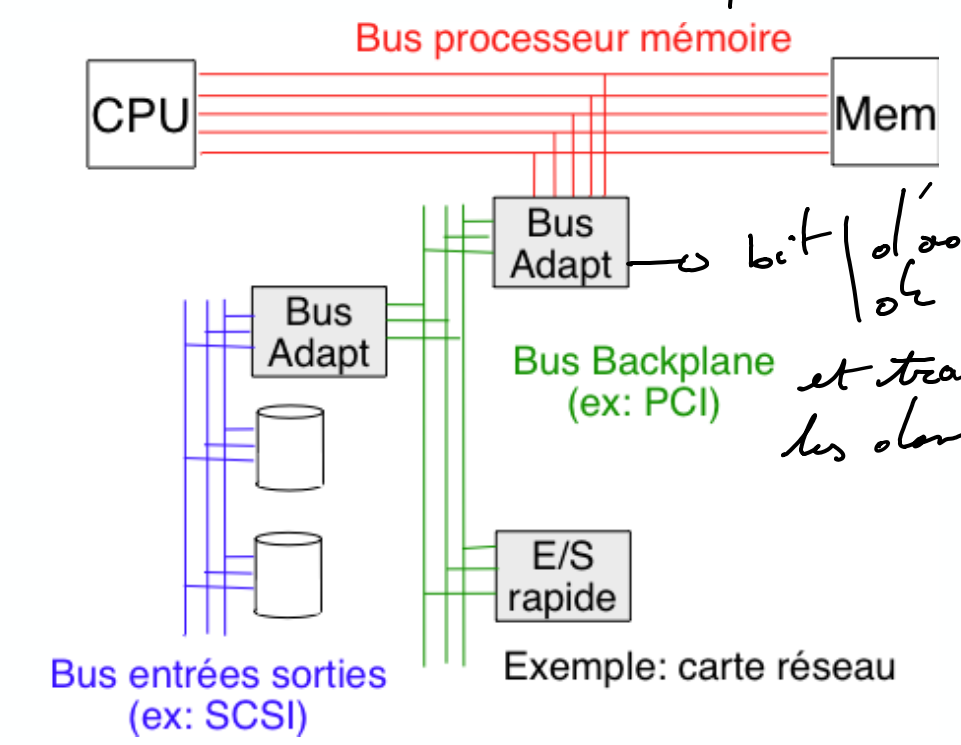
\includegraphics{image-7.png}
\caption{Alt text}
\end{figure}

\subsubsection{Technologies mémoires}\label{technologies-muxe9moires}

On a la \textbf{SRAM} (statique) et la \textbf{DRAM} (dynamique). La
SRAM est plus couteuse mais plus rapide. On va les utiliser en tandem
pour ne pas être ralenti par notre mémoire.

En effet, les cycles de CPU sont devenus extrêment cours. Encore plus
cours que ceux de la mémoire. C'est-à-dire on perdrait ce gain de
vitesse si on utilisait pas de la DRAM car on devrait attendre pour
plusieurs cycles avant d'avoir l'information.

Ces deux technologies sont dites \textbf{volatiles}. Quand plus de jus
c'est mort.

\paragraph{SRAM}\label{sram}

\begin{figure}
\centering
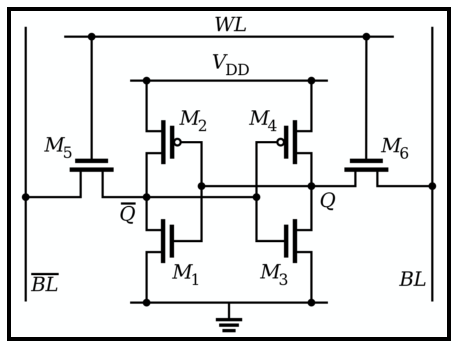
\includegraphics{image-8.png}
\caption{Alt text}
\end{figure}

On a donc de multiples bascules (6 transistor par bit (ou 4 + des
resistances)). On lit la valeur en fonction du passage ou non du
courant.

\paragraph{DRAM}\label{dram}

On stocke l'information dans des condensateurs

\begin{figure}
\centering
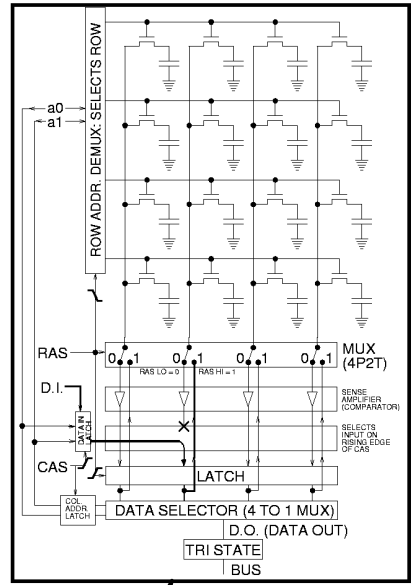
\includegraphics{image-9.png}
\caption{Alt text}
\end{figure}

La lecture des bits se fait sous forme de matrice donc si on veut lire
une valeur, on lit en réalité toute la ligne. Donc le temps pour lire 1
valeur et 64 est la même.

\begin{figure}
\centering
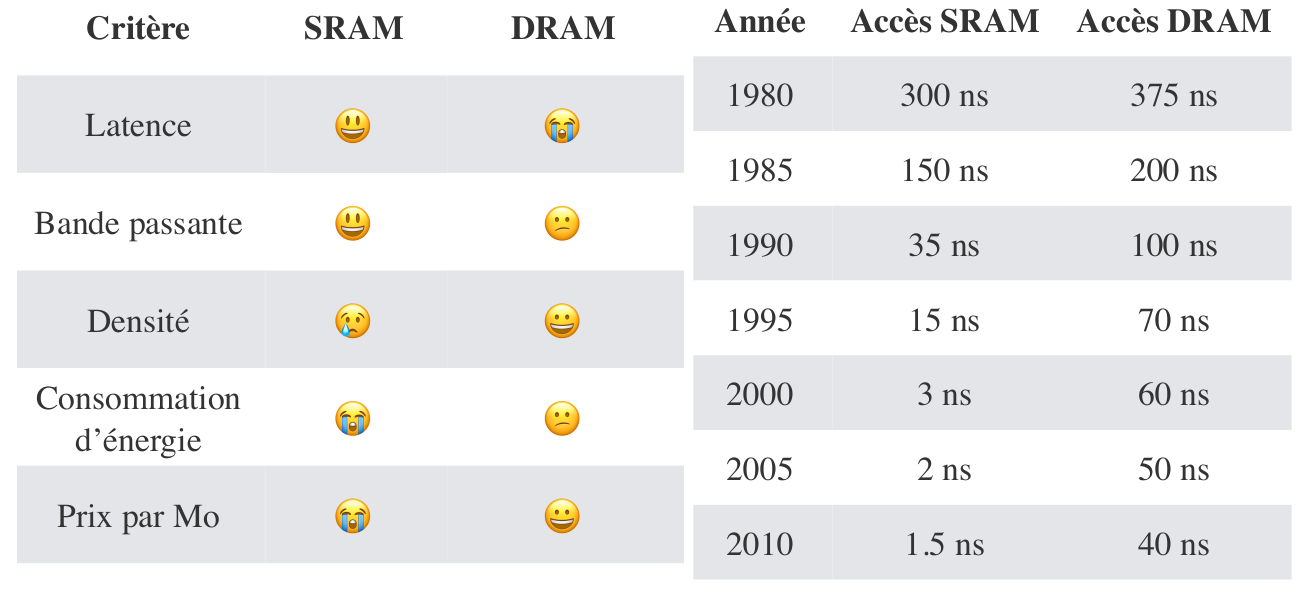
\includegraphics{image-10.png}
\caption{Alt text}
\end{figure}

On doit donc combiner un peu de SRAM coûteuse avec de la DRAM peu chère.
On utilise la SRAM comme cache.

\subsubsection{Cache}\label{cache}

Le cache interagit directement avec le Cache. On y conserve les données
récemment accédées.

\subsubsection{Localité}\label{localituxe9}

\paragraph{Temporelle}\label{temporelle}

On peut accéder à la même donnée se trouvant au même endroit, on va
souvent repasser dessus.

\paragraph{Localité}\label{localituxe9-1}

On va passer sur toutes les adresses car nos données sont juxtaposé.

\subsubsection{Hiérarchie}\label{hiuxe9rarchie}

\begin{figure}
\centering
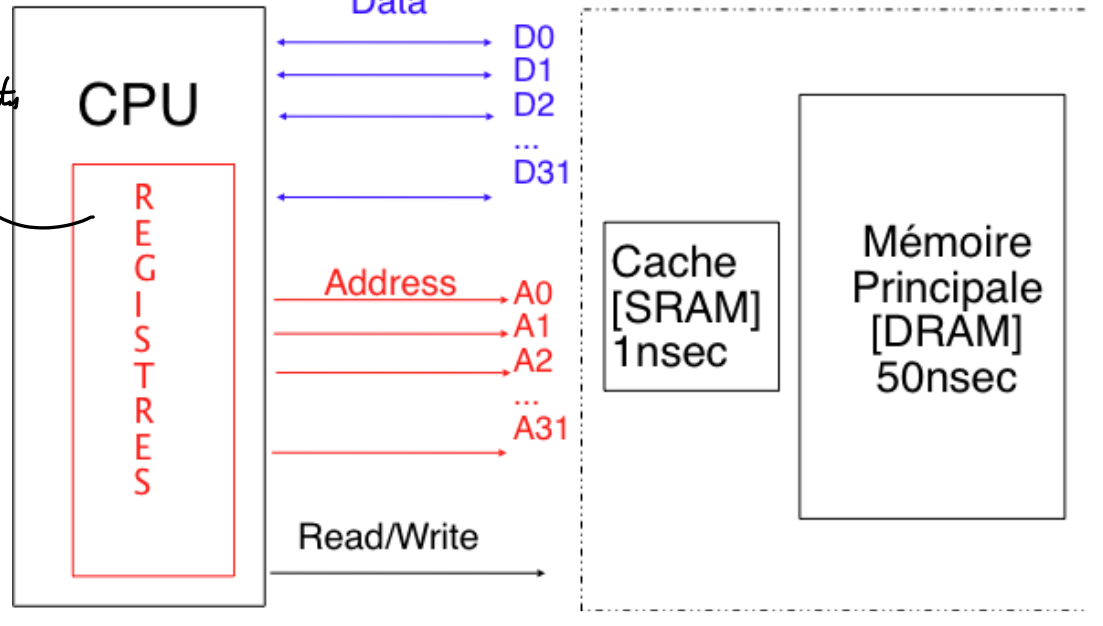
\includegraphics{image-11.png}
\caption{Alt text}
\end{figure}

\subsubsection{Fonctionnement d'un
cache}\label{fonctionnement-dun-cache}

\paragraph{Lecture}\label{lecture}

On va lire l'octet à une adresse spécifique. Si cette adresse se trouve
déjà en cache on va lire l'adresse depuis le cache.

Sinon, la mémoire cache va récupérer une copie de la mémoire à cette
adresse. On a donc toute la granularité donc 64 octets ! On sauvegarde
le tout dans le cache.

\paragraph{Écriture}\label{uxe9criture}

Si on veut écrire \texttt{A}, on va regarder si on a l'adresse de
destination en cache. On écrit directement dans le cache ou bien on doit
récupérer depuis la mémoire.

\begin{enumerate}
\def\labelenumi{\arabic{enumi}.}
\tightlist
\item
  \textbf{Write through}: écriture immédiate.
\item
  \textbf{Write back}: on écrit au moment où la ligne de cache est
  retiré du cache.
\end{enumerate}

\paragraph{Réalité}\label{ruxe9alituxe9}

On a dans un processeur 3 niveaux de caches : \texttt{L1,\ L2,\ L3}

\subsection{Jeu d'instructions IA 32}\label{jeu-dinstructions-ia-32}

Ce jeu d'instructions est 32 bits ! (donc max 4 Go de mémoire).

\subsubsection{Registres}\label{registres}

On a 8 registres génériques de \textbf{32 bits}: - \texttt{EAX} -
\texttt{EBX} - \texttt{ECX} - \texttt{EDX} - \texttt{ESI} - \texttt{EDI}
- \texttt{EBP}: gère la pile - \texttt{ESP}: gère la pile

On a 1 registres qui stocke le compteur de programme: - \texttt{EIP}

On a également des registres pour traiter les floats et double.

\subsubsection{Types de données}\label{types-de-donnuxe9es}

\begin{longtable}[]{@{}ccc@{}}
\toprule\noalign{}
Type & Taille (octets) & Suffixe assembleur \\
\midrule\noalign{}
\endhead
\bottomrule\noalign{}
\endlastfoot
\texttt{char} & 1 & b \\
\texttt{short} & 2 & w \\
\texttt{int} & 4 & l \\
\texttt{long\ int} & 4 & l \\
\texttt{void\ *} & 4 & l \\
\end{longtable}

\subsubsection{Instructions}\label{instructions}

\begin{longtable}[]{@{}
  >{\centering\arraybackslash}p{(\columnwidth - 4\tabcolsep) * \real{0.1798}}
  >{\centering\arraybackslash}p{(\columnwidth - 4\tabcolsep) * \real{0.1236}}
  >{\centering\arraybackslash}p{(\columnwidth - 4\tabcolsep) * \real{0.6966}}@{}}
\toprule\noalign{}
\begin{minipage}[b]{\linewidth}\centering
Fonctions
\end{minipage} & \begin{minipage}[b]{\linewidth}\centering
Variantes
\end{minipage} & \begin{minipage}[b]{\linewidth}\centering
Explications
\end{minipage} \\
\midrule\noalign{}
\endhead
\bottomrule\noalign{}
\endlastfoot
\texttt{mov} & \texttt{movb} & \texttt{movb\ src,\ dest}: déplace de
\texttt{src} vers \texttt{dest} pour taille 1 \\
& \texttt{movw} & \texttt{movb\ src,\ dest}: déplace de \texttt{src}
vers \texttt{dest} pour taille 2 \\
& \texttt{movl} & \texttt{movb\ src,\ dest}: déplace de \texttt{src}
vers \texttt{dest} pour taille 4 \\
\texttt{inc} & \texttt{b},\texttt{w},\texttt{l} & Incrémente la
valeur \\
\texttt{dec} & \texttt{b},\texttt{w},\texttt{l} & Décrémente la
valeur \\
\texttt{not} & \texttt{b},\texttt{w},\texttt{l} & Négation \\
\texttt{add} & \texttt{b},\texttt{w},\texttt{l} &
\texttt{add\ addition,\ dest}: ajoute à dest addition \\
\texttt{sub} & \texttt{b},\texttt{w},\texttt{l} &
\texttt{sub\ soustraction,\ dest}: soustrait à dest soustraction \\
\texttt{mul} & \texttt{b},\texttt{w},\texttt{l} & Même chose que pour
sub et add, \texttt{imul} pour les nombres signés \\
\texttt{div} & \texttt{b},\texttt{w},\texttt{l} & Division d'entiers
non-signés \\
\texttt{shl} \& \texttt{shr} & \texttt{b},\texttt{w},\texttt{l} & Shift
vers la gauche et la droite (utile en binaire) \\
\texttt{or}/\texttt{xor}/\texttt{and} & \texttt{b},\texttt{w},\texttt{l}
& Opération logique binaires avec résultat dans \texttt{dist} \\
\end{longtable}

\subsubsection{Modes d'adressage}\label{modes-dadressage}

Pour spécifier un registre, on utilise \texttt{\%eax} pour spécifier le
registre \texttt{EAX}. Pour écrire une valeur dans un registre, on fait
\texttt{\$123} pour écrire \texttt{123}.

\begin{Shaded}
\begin{Highlighting}[]
\NormalTok{movl $123, \%eax ; écris dans le registre eax }
\end{Highlighting}
\end{Shaded}

On peut faire une référence \textbf{absolue}. C'est-à-dire faire
\texttt{movl\ 0x04,\ \%eax} pour mettre dans \texttt{eax} la valeur se
trouvant à l'adresse \texttt{0x04}.

On peut être \textbf{indirect}. On peut spécifier un registre qui
contient une adresse.

\begin{Shaded}
\begin{Highlighting}[]
\NormalTok{movl (\%eax), \%ecx   ; écris dans ecx ce qui se trouve dans le registre eax.}
\end{Highlighting}
\end{Shaded}

On peut faire de l'\textbf{indirect avec base et déplacement}. On accede
à une adresse + ou - la valeur donnée. On fait \texttt{D(\%reg)} qui
permet de bouger l'adresse de D.

\begin{Shaded}
\begin{Highlighting}[]
\NormalTok{movl $0x08, \%eax    ; place la valeur 0x08 dans \%eax}
\NormalTok{movl 0(\%eax), \%ecx  ; place la valeur (0xFF) se trouvant à l\textquotesingle{}adresse}
\NormalTok{                    ; 0x08= (0x08+0) dans le registre \%ecx}
\NormalTok{movl 4(\%eax), \%ecx  ; place la valeur (0x10) se trouvant à l\textquotesingle{}adresse}
\NormalTok{                    ; 0x0C (0x08+4) dans le registre \%ecx}
\NormalTok{movl {-}8(\%eax), \%ecx ; place la valeur (0x04) se trouvant à l\textquotesingle{}adresse}
\NormalTok{                    ; 0x00 (0x08{-}8) dans le registre \%ecx}
\end{Highlighting}
\end{Shaded}

\subsubsection{\texorpdfstring{Registre de drapeaux
\texttt{eflags}}{Registre de drapeaux eflags}}\label{registre-de-drapeaux-eflags}

On a un registre spécial \texttt{eflags} qui contient des bits
``drapeau'' qui est mis à jour à l'exécution des instructions.

\begin{itemize}
\tightlist
\item
  \textbf{ZF}: indique si le résultat de la dernière opération est = à
  0.
\item
  \textbf{SF}: indique si le résultat de la dernière opération est
  \textless{} à 0.
\item
  \textbf{CF}: indique si le résultat de la dernière opération
  arithmétique \textbf{non-signé} requiert plus de 32 bits.
\item
  \textbf{OF}: indique si le résultat de la dernière opération
  arithmétique \textbf{signé} requiert plus de 32 bits.
\end{itemize}

Ce registre se met à jour mais certaines opérations ne vont pas stocker
le résultat: - \texttt{cmp}: équivalent de \texttt{sub} - \texttt{test}:
équivalent de \texttt{and}

Pour récupérer la valeur des drapeaux on utilise \texttt{set}. -
\texttt{sete}: \textbf{ZF} - \texttt{sets}: \textbf{SF} - \texttt{setg}:
\texttt{\textasciitilde{}SF\ \&\ ZF} en gérant dépassement
test\textgreater{} - \texttt{setl}: \textbf{SF} et gérant le dépassement
test\textless=

\paragraph{Exemples}\label{exemples}

Jetez un œil au
\href{https://sites.uclouvain.be/SystInfo/notes/Theorie/Assembleur/memory.html}{syllabus}.

\subsubsection{Saut}\label{saut}

On va modifier la valeur du \textbf{compteur de programme}
\texttt{\%eip}.

\paragraph{Inconditionnel}\label{inconditionnel}

On fait simplement \texttt{jmp\ {[}etiquette{]}}. On va donc sauter
jusqu'à une étiquette. On peut aussi sauter à une adresse mémoire via
\texttt{jmp\ *\%eax} (saute à l'instruction se trouvant à l'adresse
mémoire dans EAX).

\paragraph{Conditionnel}\label{conditionnel}

La comparaison compare avec la dernière valeur en référence.

\begin{itemize}
\tightlist
\item
  \texttt{je}: Saut si égal
\item
  \texttt{js}: Saut si négatif
\item
  \texttt{jg}: Saut si strictement supérieur à
\item
  \texttt{jge}: Saut si supérieur ou égal à
\item
  \texttt{jl}: Saut si strictement inférieur à
\item
  \texttt{jle}: Saut si inférieur ou égal à
\end{itemize}

Pour les négations, on rajoute un \texttt{n} après \texttt{j}.

\subsubsection{Manipulation de la Pile}\label{manipulation-de-la-pile}

Comme dit plus haut, la pile est stocké dans le registre \texttt{\%esp}.

\paragraph{Opérations}\label{opuxe9rations}

\begin{itemize}
\tightlist
\item
  \texttt{pushl\ \%reg}: place le contenu \texttt{\%reg} au somment de
  la pile. Décrémente la taille du registre \texttt{\%esp} de 4.
\item
  \texttt{popl\ \%reg}: retire le mot de 32 bits du sommet de la pile et
  le place dans \texttt{\%reg}. Incrémente la taille du registre
  \texttt{\%esp} de 4.
\end{itemize}

\subsubsection{Fonctions}\label{fonctions}

On a comme en Oz des procédures qui sont des fonctions sans valeur de
retour.

\paragraph{Appel}\label{appel}

\begin{enumerate}
\def\labelenumi{\arabic{enumi}.}
\tightlist
\item
  Sauver l'adresse de l'instruction qui suit l'appel de fonction
\item
  Positionner le compteur de programme à la première instruction de la
  fonction appelée
\item
  Exécuter la fonction
\item
  Positionner le compteur de programme à l'adresse qui suit l'appel,
  précédemment sauvée
\end{enumerate}

L'instruction \texttt{call} combine l'étape 1 et 2. \texttt{ret} réalise
l'étape 4. À savoir que \texttt{call} et \texttt{ret} modifie la pile
(donc \texttt{\%esp}).

\begin{Shaded}
\begin{Highlighting}[]
\NormalTok{increase:     ; étiquette de la première instruction}
\NormalTok{            movl  g,  \%eax}
\NormalTok{            addl  h,  \%eax}
\NormalTok{            movl  \%eax, g}
\NormalTok{            ret}
\NormalTok{init\_g: }
\NormalTok{            movl  $1252,  g}
\NormalTok{            ret}
\NormalTok{main: }
\NormalTok{            (...)}
\NormalTok{            calll init\_g}
\NormalTok{A\_init\_g:   calll increase}
\NormalTok{A\_increase: movl  $0, \%eax}
\NormalTok{            addl  $12, \%esp}
\NormalTok{            ret}
\NormalTok{g:}
\NormalTok{      .long 0}
\NormalTok{h:}
\NormalTok{      .long 2}
\end{Highlighting}
\end{Shaded}

\paragraph{Avec Arguments}\label{avec-arguments}

On place les arguments dans la pile. On passe donc les arguments par
\textbf{valeur}. On met donc l'adresse de retour sur le sommet de la
pile puis le premier, second, \ldots{}

Pour modifier les registres \texttt{\%eax}, \texttt{\%ecx} et
\texttt{\%edx}, il faut faire une copie de sauvegarde.

Pour modifier les registres \texttt{\%ebx}, \texttt{\%edi} et
\texttt{\%esi}, il faut copier puis restaurer. (qu'un convention)

\paragraph{Valeur de Retour}\label{valeur-de-retour}

On stocke les valeurs de retour dans le registre \texttt{\%eax} par
convention.
